\documentclass[
  accentcolor=tud1c,	% Color theme for TUD corporate design
  colorbacktitle,		% Titlepage has colored background for title area
  inverttitle,			% Font color of title on titlepage is inverted
  german,
  twoside
]{tudexercise}

\usepackage[ngerman]{babel}
\usepackage{units}
\usepackage{hyperref}
\usepackage{booktabs}
\usepackage[utf8]{inputenc}
\usepackage{algorithm2e}
\usepackage{paralist}

\definecolor{commentgreen}{RGB}{50,127,50}


\usepackage{listings}
\lstloadlanguages{C++,[gnu]make}
\lstset{language=C++}
\lstset{captionpos=b}
\lstset{tabsize=3}
\lstset{breaklines=true}
\lstset{basicstyle=\ttfamily}
\lstset{columns=flexible,keywordstyle=\color{purple},stringstyle=\color{blue},commentstyle=\color{commentgreen}}
\lstset{literate=%
	{Ö}{{\"O}}1
	{Ä}{{\"A}}1
	{Ü}{{\"U}}1
	{ß}{{\ss}}2
	{ü}{{\"u}}1
	{ä}{{\"a}}1
	{ö}{{\"o}}1
	{'}{{\textquotesingle}}1
}

\lstnewenvironment{lstmake} %
{\lstset{language=[gnu]make}} %
{}

\parindent0pt
\parskip2ex


\newcommand{\superscript}[1]{\ensuremath{^{\textrm{#1}}}}
\newcommand{\subscript}[1]{\ensuremath{_{\textrm{#1}}}}

\newcommand{\cppSetTitle}{
	\title{Übung zum\linebreak[1]C/C++-Praktikum\linebreak[1] Fachgebiet Echtzeitsysteme}
	\subtitle{Übungen für den \tag{}. Tag}
}

\newcommand{\cppSetHeaderAndMakeTitle}{
	\begin{examheader}
		\textmb{Übung zum C/C++-Praktikum - Tag \tag{}}
	\end{examheader}
	\maketitle
}

\newcommand{\tag}{6}
%\setcounter{section}{18}

\cppSetTitle

\begin{document}

\cppSetHeaderAndMakeTitle 


\noindent Heute ist es an der Zeit, Ihr neu erlerntes Wissen bei der Programmierung von Microcontrollern umzusetzen.
Du hast hierbei die freie Wahl - die beiden folgenden Aufgaben sind lediglich Beispiele für Programme.

\section{Pong}


Erstellen Sie das Spiel Pong.
Zwei Gegner sollen je einen Balken (Rechteck) am linken oder rechten Rand des Spielfeldes mit den Schiebereglern steuern können, um einen Ball (ein Quadrat) im Spiel zu halten.
Erreicht der Ball den linken oder rechten Rand des Spielfelds, so bekommt der Spieler auf der anderen Seite einen Punkt.
Gewonnen hat der Spieler, der zuerst 3 Punkte hat.
Die aktuelle Punktzahl beider Spieler soll auf der 7-Segment-Anzeige ausgegeben werden.
\begin{center}
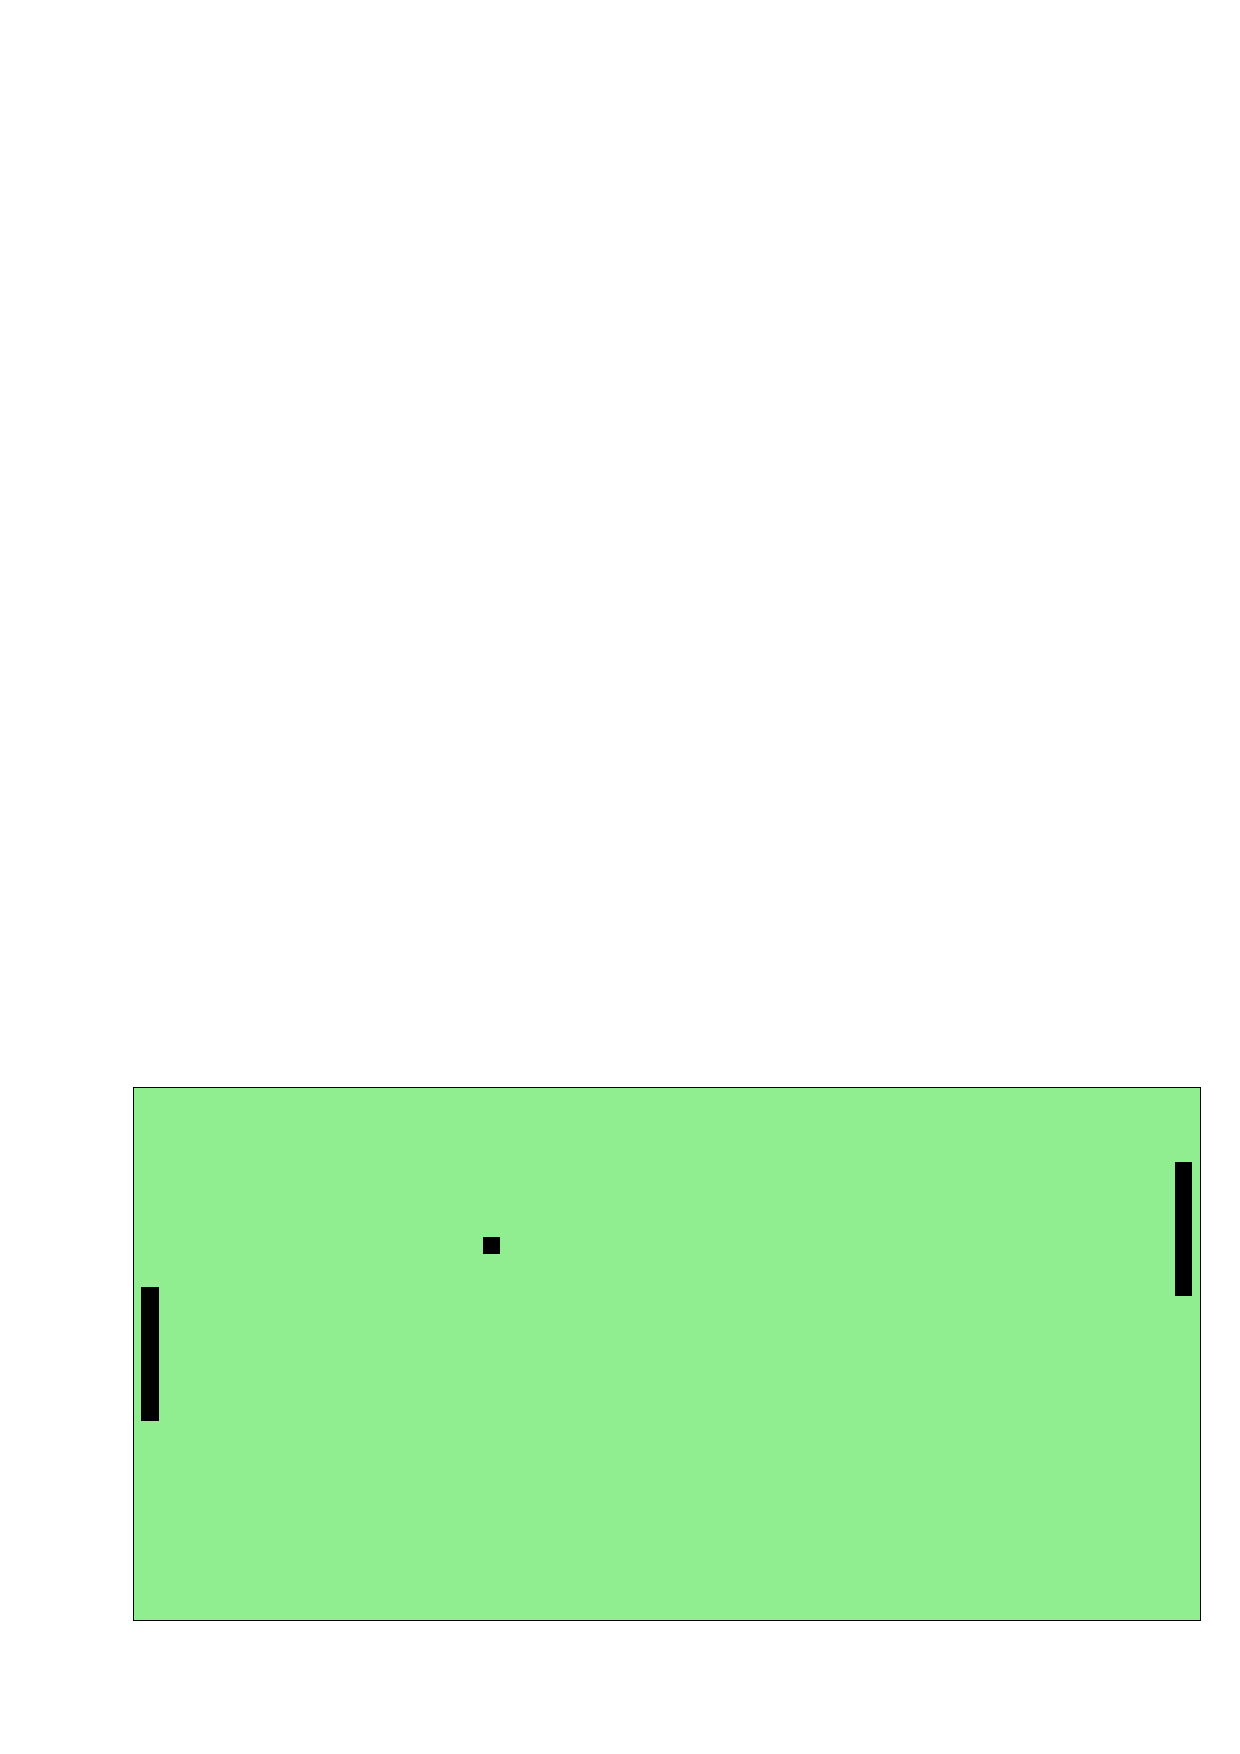
\includegraphics[scale=0.4]{pong}
\end{center}
Hinweise:
\begin{itemize}
\item Der Ball wird am oberen und unteren Rand sowie an den Balken der Spieler \glqq{}reflektiert\grqq{} -- verlässt also niemals das Spielfeld.
\end{itemize}

\section{Game of Life}

Implementiere das \glqq{}Game of Life\grqq{}\footnote{siehe auch \url{http://de.wikipedia.org/wiki/Conways_Spiel_des_Lebens}}.
Das Display von 128\,x\,64 Pixel ist das Spielfeld.
Jedes Pixel steht für eine Zelle, die \textit{tot} (grün) oder \textit{lebendig} (schwarz) ist.
Jede Zelle hat acht Nachbarzellen, die ebenso tot oder lebendig sein können.
Zu Beginn gibt es eine vordefinierte Anfangsgeneration.
Durch festgelegte Regeln wird die nachfolgende Generation ermittelt.\\
Die Spielregeln lauten:
\begin{itemize}
\item Eine \textbf{lebende Zelle} \dots
\begin{itemize}
\item \dots mit 1 oder 0 lebenden Nachbarn stirbt aus Einsamkeit.
\item \dots mit 4 oder mehr lebenden Nachbarn stirbt wegen Übervölkerung.
\item \dots mit 2 oder 3 lebenden Nachbarn bleibt am Leben.
\end{itemize}
\item Eine \textbf{tote Zelle} mit genau 3 lebenden Nachbarn wird in der nächsten Generation geboren werden, andernfalls bleibt sie tot.
\end{itemize}
Da das Spielfeld begrenzt ist soll es torusförmig aufgebaut werden (alles, was am unteren Rand des Spielfelds verschwindet, kommt oben wieder heraus -- das Gleiche gilt für den linken und rechten Rand). 
Verwende als Anfangsgeneration entweder eine zufällige Population oder eine der folgenden Figuren:
\begin{center}
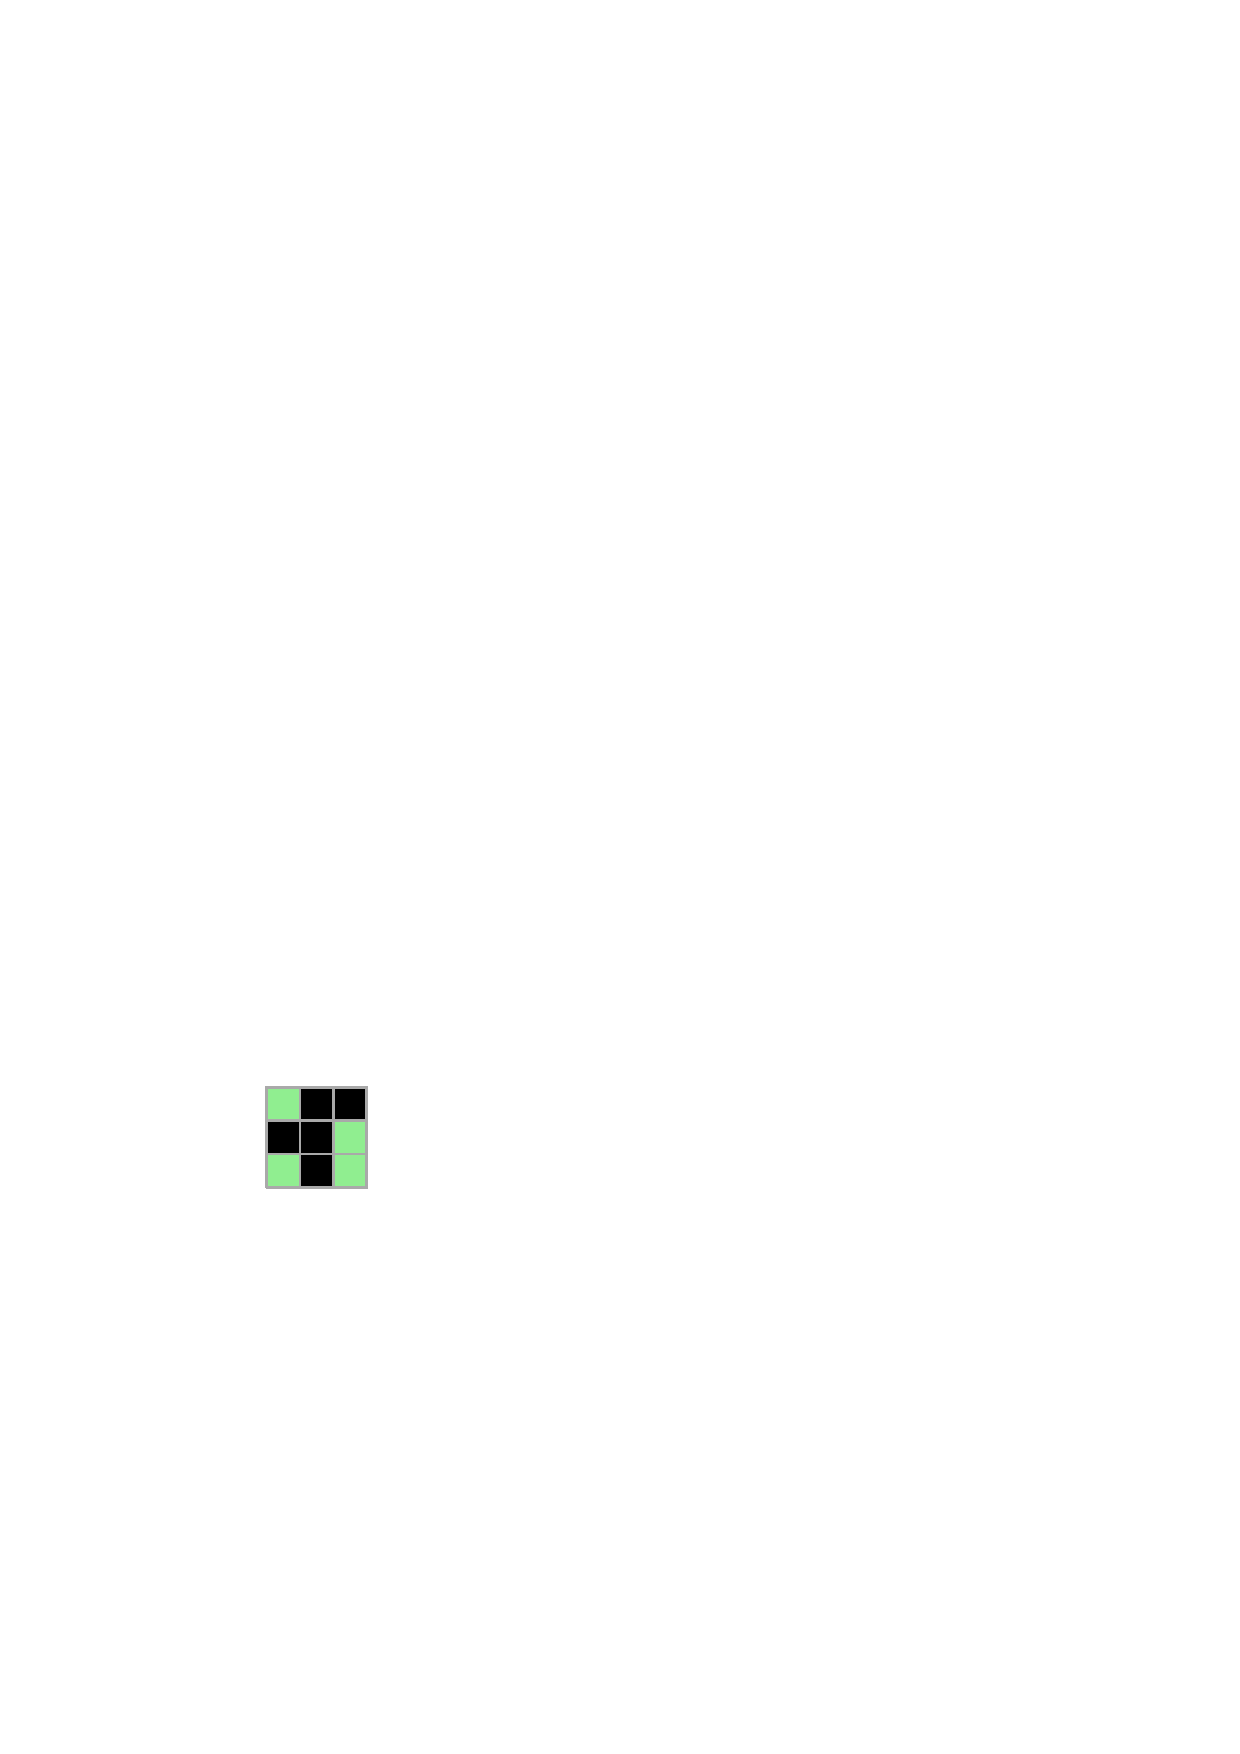
\includegraphics[scale=1]{gol_init1}
\hspace{5mm}
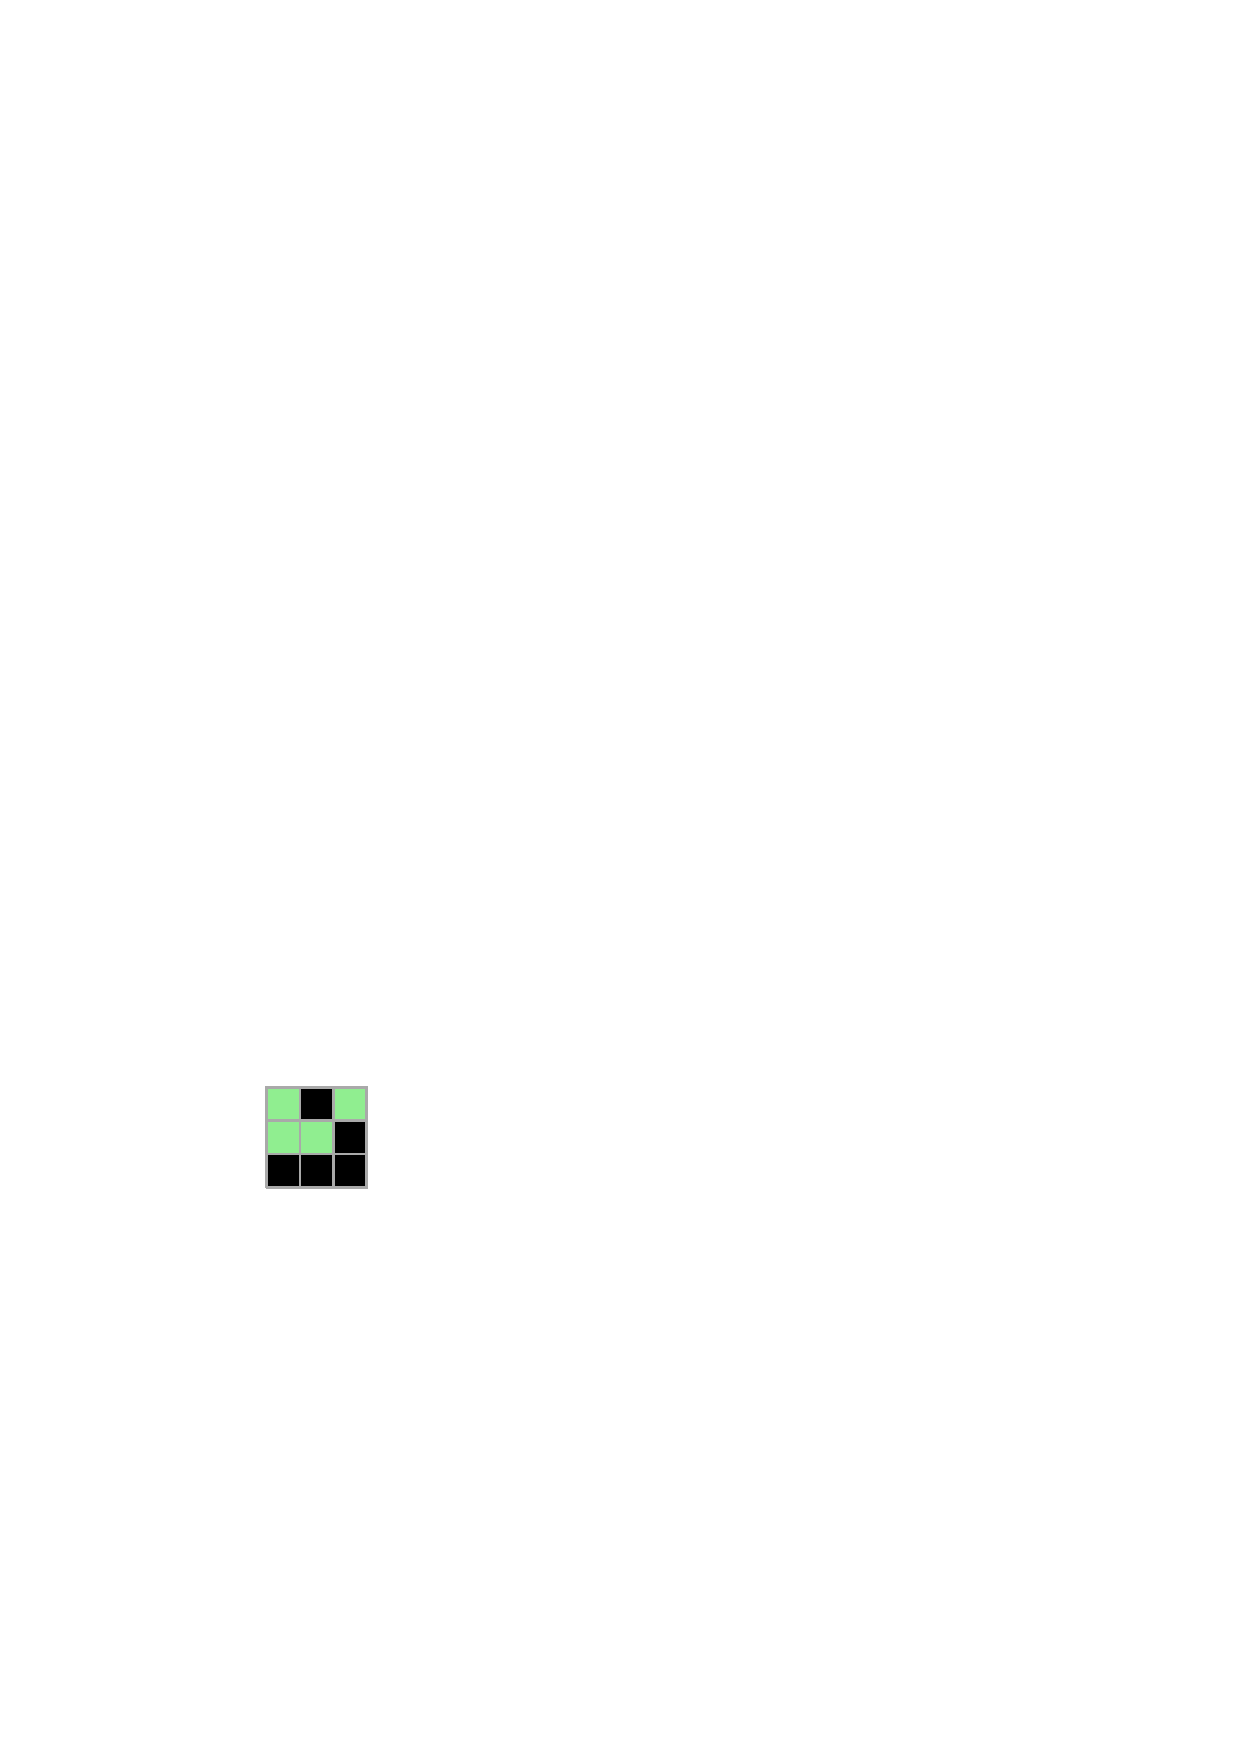
\includegraphics[scale=1]{gol_init2}
\hspace{5mm}
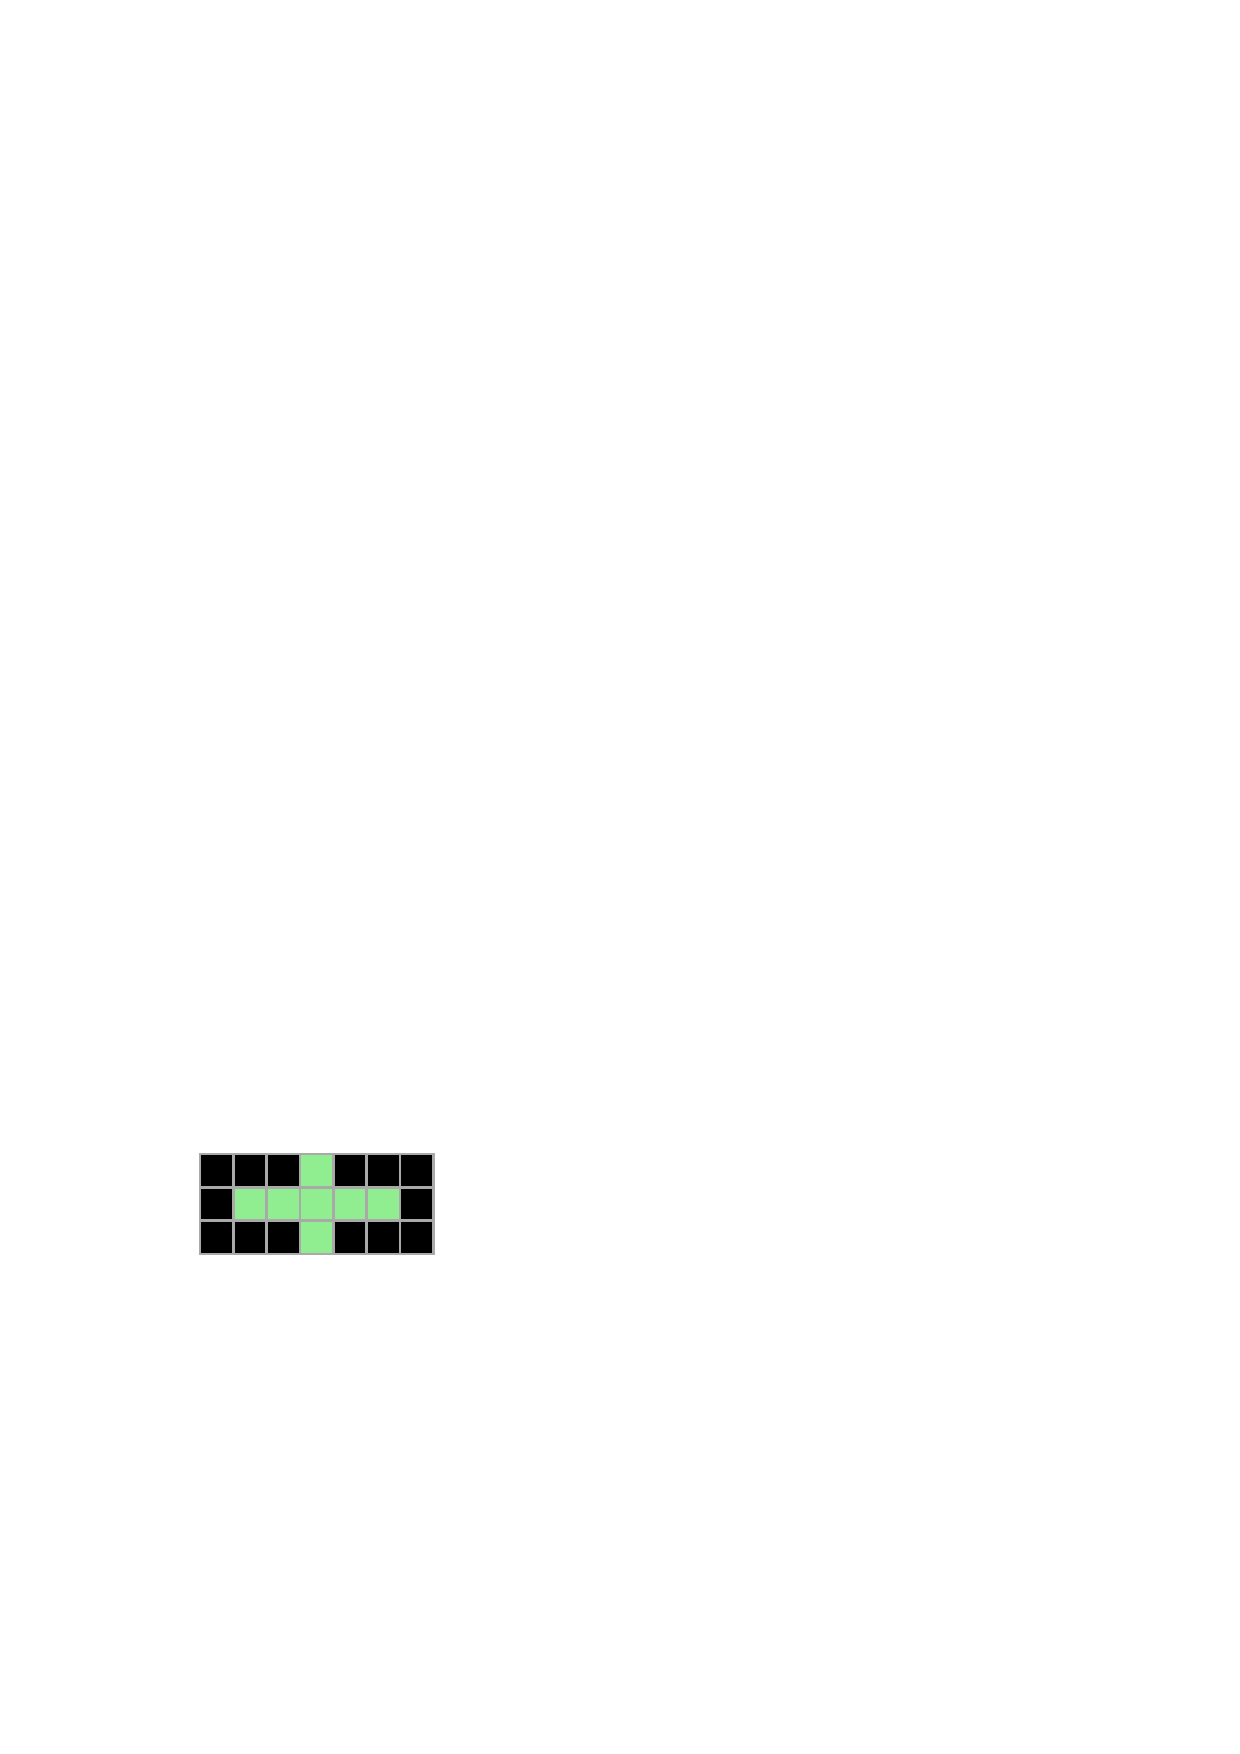
\includegraphics[scale=1]{gol_init3}
\end{center}
Hinweise:
\begin{itemize}
\item Verwende als Spielfeld folgendes mehrdimensionales Array:
\texttt{unsigned char gamefield[128][8];}
\item Ein weiteres mehrdimensionales Array bietet sich an, um die zukünftige Generation erzeugen zu können.
\item Achte beim torusförmigen Feld unbedingt darauf, dass du nicht über die Grenzen des Spielfelds hinaus zugreifst!
\end{itemize}

\section{Weitere Ideen}

Der Fantasie sind keine Grenzen gesetzt:

\begin{itemize}
\item Asteroids\\
\begin{center}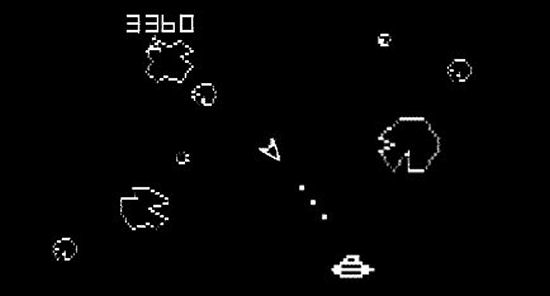
\includegraphics[width=.5\textwidth]{asteroids.png}\end{center}
\item Pacman\\
\begin{center}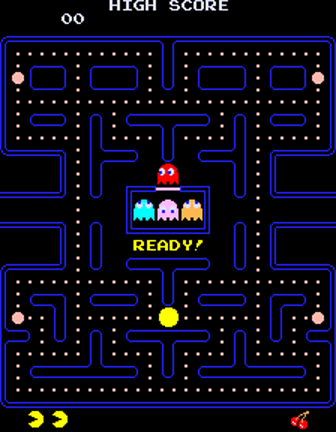
\includegraphics[width=.3\textwidth]{pacman.png}\end{center}
\item Labrinth
\begin{center}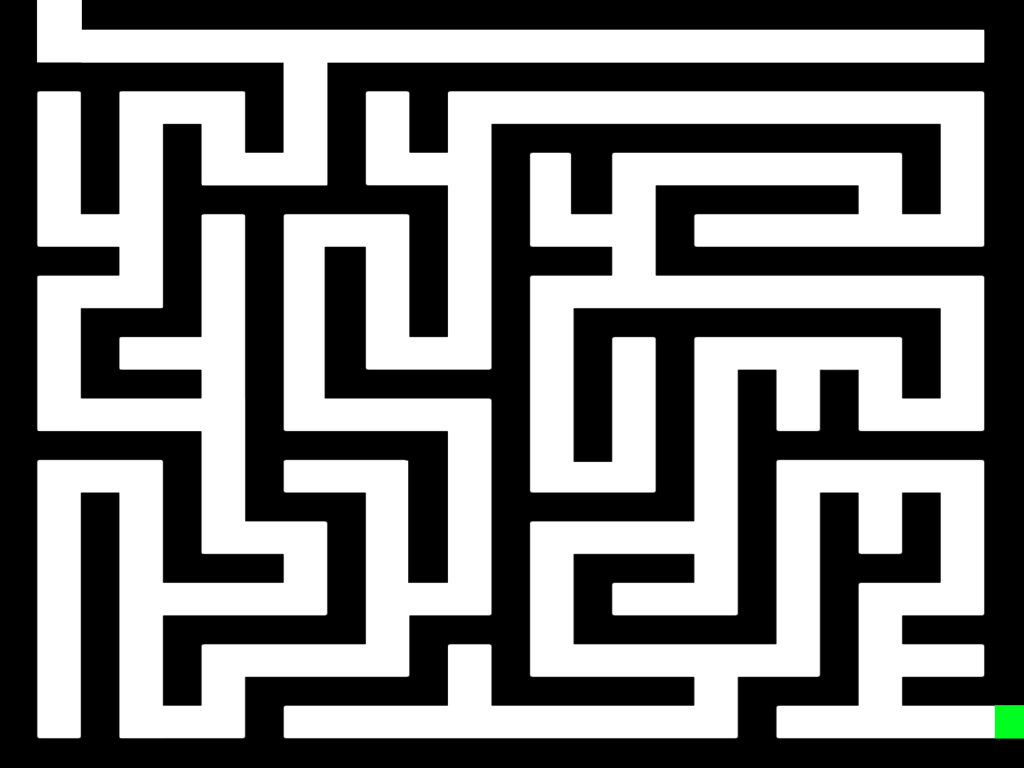
\includegraphics[width=.4\textwidth]{maze.png}\end{center}
\item \glqq Ausweichspiele\grqq{} 
\begin{center}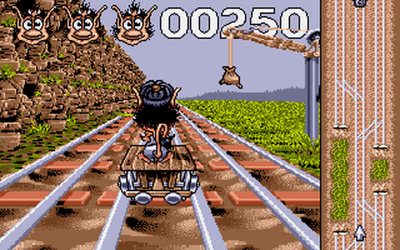
\includegraphics[width=.4\textwidth]{hugo.png}\end{center}
\item \dots
\end{itemize}



\end{document}
